\documentclass{article}
\usepackage{graphicx}
\usepackage{wrapfig}
\usepackage{subcaption}
\usepackage[margin=1in]{geometry}
\usepackage{amsmath} % or simply amstext
\usepackage{amssymb}
\usepackage{siunitx}
\usepackage{booktabs}
\usepackage[export]{adjustbox}
\newcommand{\angstrom}{\textup{\AA}}
\newcommand{\colormap}{jet}  % colorbar to use
\usepackage{cleveref}
\usepackage{booktabs}
\usepackage{gensymb}
\usepackage{float}

%MRS: better to have the first outline shorter to iterate more quickly!
%BJC1: right, this one has been in the works for a while now. Wrote the anomalous diffusion methods a long time ago

%MRS: better to have a title that described a finding, rather than the
%approach used.  But we may need to wait a bit further until we can decide on a finding.
%MRS: also 'stochastic modeling' is pretty vague.  should be more precise. 
\title{Using Stochastic Modeling to Predict Long Timescale Transport Behavior of Solutes in an H\textsubscript{II} Phase Lyotropic Liquid Crystal Membrane}
%MRS: we should discuss whether Chris Calderon would be on this one.  I would guess no, but I don't know for sure. 
%BJC1: Yea maybe Chris as an acknowledgement on this one. He didn't directly contribute anything other than pointing
%me towards Greg Morrin who pointed me towards useful anomalous diffusion literature.
\author{Benjamin J. Coscia \and Michael R. Shirts} 

\begin{document}

  \graphicspath{{./figures/}}
  \maketitle

  \section{Introduction}
  %BJC: obviously this section will get beefed up
  We need highly selective membranes in order to perform efficient separations. \\

  \noindent Amphiphilic molecules are capable of self-assembling into ordered nanostructures.\\

  Lyotropic liquid crystals are a class of amphiphilic molecules that can be cross-linked
  into mechanically strong membranes.
  \begin{itemize}
  	\item H\textsubscript{II} phase lyotropic liquid crystals have densely packed, uniform
	sized pores and have the potential to disrupt conventional membrane separation
	techniques by being selective based not only on size and charge, but on chemical
	functionality as well.
	\item Q\textsubscript{I} phase LLCs consist of a tortuous network of 3D interconnected
	pores. They are easier to make.
  \end{itemize}

  We can only learn so much from experiment. MD can give us mechanistic insights with
  atomistic resolution so that we can intelligently design new membranes for 
  solute-specific separations.\\

  \noindent In our previous work, we studied the transport of 20 small polar molecules
  in an H\textsubscript{II} phase LLC membrane.
  \begin{itemize}
    \item In general, we observed subdiffusive transport behavior characterized by 
    intermittent hops separated by periods of entrapment.
    \item We identified three mechanisms responsible for the solute trapping behavior:
    entanglement among monomer tails, hydrogen bonding with monomer head groups, and
    association with sodium counter ions.
  \end{itemize}

  Unfortunately, the timescales that we can simulate with MD are insufficient to be
  able to make well-converged predictions of macroscopic transport properties 
  traditionally used to characterize membranes in the lab. \\
  \begin{itemize}
    \item However, if we use descriptive stochastic models that sufficiently capture solute
    dynamics, then we could project long timescale behavior in addition to gaining
    a deeper understanding of solute behavior on short timescales.
  \end{itemize}
  
  \noindent Researchers have developed a rigorous theoretical foundation for describing
  the motion of particles exhibiting non-Brownian, or anomalous, transport behavior.
  \begin{itemize}
    \item The tools introduced by fractional calculus are instrumental to this theory. 
    \item They allow us to generalize the normally linear diffusion equation to fractional
    derivative orders, providing descriptions of a much more diverse set of behavior. \cite{klages_anomalous_2008} % diverging from the relatively simple Brownian model.
%    \item They facilitate proof of the relationship between the observed growth of a
%    particle's mean squared displacement and underlying dwell times 
%    \item In the absence of an external potential or complicated boundary conditions, 
%    one can define random walk based on independent hop length and dwell time 
%    distributions and arrive at any type of diffusive behavior. 
  \end{itemize}
  
  % BJC1: moved from methods
  \noindent Three well-known classes of behavior leading to anomalous subdiffusion are 
  continuous time random walks (CTRW), fractional Brownian motion
  (FBM) and random walks on fractals (RWF).\cite{meroz_toolbox_2015}
  \begin{itemize}
    \item The theory is frequently used to describe single particle trajectories
    \item A CTRW is characterized by a distribution of hop lengths and 
    dwell times, where each each hop is characterized by independent random draws from 
    each distribution.\cite{montroll_random_1965,morrin_three_2018}
    \item FBM is common in crowded, viscoelastic environments where each jump comes 
    from a Gaussian distribution but is anti-correlated to its previous 
    step.~\cite{mandelbrot_fractional_1968,jeon_fractional_2010,banks_anomalous_2005}
    \item An RWF is imposed by a system's geometry. Systems with tortuous pathways and dead
    ends cause anti-correlated motion.\cite{meroz_toolbox_2015,neusius_subdiffusion_2008}
    \item The processes described above can happen alone or in combination. 
    \item Meroz and Sokolov suggested a decision tree for determining which subdiffusive
    mechanisms apply to a system, adapted in Figure X. 
    \item Of course, more complicated variations on these models can arise which we 
    will incorporate as needed.	  % BJC1: e.g. fractional levy motion or langevin with levy noise
  \end{itemize}
  
  % BJC1: Flow chart here
  
  While elegant, pure anomalous diffusion theory may in some cases give only a qualitative
  understanding of transport mechanisms.
  \begin{itemize}
    \item Complex temporal relationships in between hops may have a significant effect on the average MSD
    \item Inhomogeneity of a medium or multiple types of interactions may lead to a number of
    distinct diffusive regimes. 
    \item In this case, a state based model may be useful. 
  \end{itemize}
  
  \noindent We can use the observations of transport from our previous work in order to create 
  state-based models.
  \begin{itemize}
  	\item We know that dynamics differ between solutes moving inside the pores and 
  	in the tails.
  	\item We can use the anomalous diffusion approach to model to our data as a 
  	function of radial distance from the closest pore center.
  	\item Alternatively, we can abandon the anomalous diffusion theory and adapt the 
  	methods of Markov state modeling.
  \end{itemize}

  % moved parts of method to here.
  Markov state models (MSMs) are a popular class of models used to project long timescale
  behavior of molecules based on molecular simulation trajectories by identifying
  different dynamical modes and quantifying the rates of transitions between them.
  \begin{itemize}
    \item MSMs are frequently used to study systems with slow dynamics, such as protein 
    folding.~\cite{snow_how_2005,chodera_automatic_2007}
    \item Researchers typically aim to come up with a low dimensional 
    representation of the system based on features which preserve the process
    kinetics.
    \item This still often results in thousands of distinct states. 
  \end{itemize}
  
  In this work we attempt to model the long timescale behavior of the four 
  fastest moving solutes studied in our previous work.
  \begin{itemize}
    \item Specifically, we study methanol, urea, ethylene glycol and acetic acid
    \item In addition to moving quickly, these solutes have a range of chemical
    functionality and experience each of the three trapping mechanisms to different
    degrees.
    \item It is our goal to reproduce the MSDs exhibited by each solute on MD timescales
    and then to project the long-term dynamics of each solute. 
    \item We explore two modeling approaches
%  	\item The third uses an infinite hidden Markov model (iHMM), an unsupervised machine
%  	learning algorithm which groups solute behavior into different dynamical states.
  	% BJC: somewhere emphasize that this last approach is powerful since it doesn't 
  	% require anything different in systems with more complex geometries (i.e. QI)
  \end{itemize}
  
  Our first approach is based on the anomalous diffusion literature, applying the 
  mathematical formalism describing subdiffusive transport to observed solute 
  trajectories.
  \begin{itemize}
    \item We determine the most likely subdiffusive mechanisms at play using the 
    flow chart in figure X. 
    \item We then fit anomalous diffusion models in two ways: First, based on a
    single set of parameters. Second, we use a two-state approach incorporating
    two sets of parameters based on a solute's radial distance from the pore center. 
  \end{itemize}
  
  The second approach adapts the MSM framework to a relatively small set of known 
  states based on the three observed solute trapping mechanisms.
  \begin{itemize}
    \item We extend the framework to include dynamics between jumps. 
    \item That is we incorporate the magnitude and temporal dependence of the 
    time series fluctuations between each transition to a different state. 
    \item Temporal dependence has a significant influence on mean squared displacement.
  \end{itemize}

  % BJC: I've been trying to understand the following justification a bit more. Does it
  % rely on the MSD becoming linear so we can get experimentally diffusion constants? Is
  % it just to try and reduce uncertainty in our MSD predictions? What can we learn from
  % long stochastic simulations that we can't learn from the shorter simulations.
  % BJC: To me the value in this is gaining a deeper mechanistic understanding by 
  % putting things in terms of easily interpreted equations.
  % BJC: Maybe it's just a combination of both.

  % MRS: They way to think about it, I think, is that the simplest
  % assumption is the the transport mechanism is simple diffusion;
  % uncorrelated random jumps due to molecular collisions. If you make
  % that assumption, you get MSD linear in time.  So that's IS a
  % stochastic process, but not a very complex one. To make long
  % timescale predictions, we need to increase the detail.  Is that
  % what you are referring to? Not sure if I answered the question . . . 
  % BJC1: Yea, I see what you're saying. Just not sure what else the long
  % timescale will tell us that we can't learn from short ones. Probably 
  % better to talk about this in person. 

%  We can use the observed mechanisms in order to choose a stochastic model of
%  sufficient complexity One can project long timescale solute behavior by modeling transport as a
%  stochastic process.
%  %MRS: as above, simple diffusion is stochastic, just not very complex.  So we want to add appropriate complexity.
%  \begin{itemize}
%    %MRS: best talk about these mechanisms in terms of the
%    %mathematical models they capture.  But I don't know that it's
%    %necessary to review all of them.  
%  
%    %It may be a better approach to start from the features of the
%    %problem (i.e. certain mechanisms) and choose the model (of the
%    %existing choices) that is appropriate for those mechanisms.
%    %I.e. diagnose first, then choose, rather than just applying a
%    %list of models useful in other field's timeseries. Let me know if that makes sense;
%    %I think how the methods applied are selected is a key to solve the problem.
%
%    \item Various disciplines study this type of problem in a number of ways.
%    \item In the simulation literature, most start by measuring mean squared 
%    displacement (MSD), as we did previously.  % This doesn't quite fit the thesis
%    \item Due to the short time scales most people can feasibly simulate, the MSD 
%    does not give a complete picture of what happens long-term, other than hinting
%    at types of mechanisms that could lead to the curve's shape.
%    %MRS: I'd say that MSD is too simple compared to what is going on mechanistically, but it's fundamentally the same idea.  
%    \item mean first passage time?
%    \item Markov state models are popular with researchers of proteins which have 
%    many dynamical states occurring over multiple time scales.
%    \item The anomalous diffusion literature explains the shape of MSD curves based
%    on rigorous mathematical representations of transport mechanisms. This field is
%    heavily used in analysis of single particle tracking experiments.
%    \item Finally, the financial literature tackles similar problems from a more 
%    general time series perspective. Their primary focus is towards predictions of
%    stock market returns and volatility but their methods are widely applicable to
%    modeling time series that exhibit a range of behavior.
%  \end{itemize}

  \section{Methods}
    
  We ran all MD simulations and energy minimizations using GROMACS 2018. We  % needs gromacs citations
  performed all post-simulation trajectory using python scripts which are available
  %MRS: eventually want to say what scripts were used to do what, but that is not at the outline stage!
  %BJC1: I usually put a table like that in the SI. Is that sufficient?
  online at \\ \texttt{https://github.com/shirtsgroup/LLC\_Membranes}.

  \subsection{Molecular Dynamics Simulations}

  We studied transport of solutes in the H\textsubscript{II} phase using an
  atomistic molecular model of four pores in a monoclinic unit cell with 
  10 \% water by weight. (See Figure tbd)
  \begin{itemize}
    \item Approximately one third of the water molecules occupy the tail region 
    with the rest near the pore center.
    \item We chose to study the 10 wt \% water system because solutes move 
    significantly faster than in the 5 wt \% system studied previously.
    \item Appropriate stochastic modeling requires that solutes sample the 
    accessible mechanisms with representative probability.  %BJC1: incorporated suggested phrasing
  \end{itemize}
  
  We chose to study a subset of 4 of the fastest moving solutes from our previous
  work: methanol, acetic acid, urea and ethylene glycol.
  \begin{itemize} 
    \item In addition to exploring membrane structural space the most, these solutes
    have a relatively diverse set of chemical functionality.   
    %MRS: do the solutes also have some diversity of mechanisms (that were observed previously?)
    %BJC1: Yes. Need to put following into words
    %BJC1: Ranking of time spent in pore region: AcOH > EG > URE > MeOH  (spans 4th most to 3rd least)
    %BJC1: All have high hop frequency which is consistent with fast motion
    %BJC1: Hbonding: Urea barely hbonds. AcOH and EG hbond a lot. AcOH has highest hbond lifetime of all 20 solutes. MeOH on par with all other simple alcohols
    %BJC1: Sodium Association: Urea coordinates with sodium the most of all 20 solutes. AcOH, EG, MeOH spread out of rest of range. Lifetime similar 
    \item For each solute we created a separate system and to each system we
    added 6 solutes per pore for a total of 24 solutes.
    \item This number of solutes per pore provides a balance of a low 
    degree of interaction between solutes and sufficient amount of data from
    which to generate statistics on the time scales which we simulate.
    \item Further details on the setup and equilibration of these systems can
    be found in our previous work.\cite{coscia_chemically_2019}
  \end{itemize}
  
  \noindent We extended the 1 $\mu$s simulations of our previous work to 5 $\mu$s in order
  to collect ample data.
  \begin{itemize}
    \item We simulated the system with a time step of 2 fs at a pressure of 1 bar
    and 300 K controlled by the Parinello-Rahman barostat and the v-rescale thermostat
    respectively.
    \item We recorded frames every 0.5 ns
  \end{itemize}

  % MRS: you intend this to be a separate model than the above?  If so, make clearer.
  % BJC1: renamed, is that what you meant?
  \subsection{The Anomalous Diffusion Model}\label{method:model_sFBM}

  Solutes in this system exhibit subdiffusive behavior, a type of anomalous diffusion.
  \begin{itemize}
  %MRS: you would probably want to be clear what the mechanistic reasons for for anomalous diffusion: 
  %want to talk about why, given the mechanisms you would consider. 
  %BJC1: could go through flow chart
  	\item During an anomalous diffusion process, the mean squared displacement (MSD)
  	does not grow linearly with time, rather it follows a power law of the form:
	\begin{equation} 
	\langle x^2(t) \rangle = K_{\alpha}t^\alpha
	\label{eqn:msd_form}
	\end{equation} 
	where $\alpha$ is the anomalous exponent and $K_\alpha$ is the
	generalized diffusion coefficient.
	\item A value of $\alpha < 1$ indicates a subdiffusive process, while values of
	$\alpha = 1$ and $\alpha > 0$ are characteristic of Brownian and superdiffusive
	motion respectively.
  \end{itemize}

  \noindent We analyzed both the ensemble-averaged and time-averaged MSDs
  of the simulated trajectories.
  \begin{itemize}
    %MRS: describe the physical situations in which one would want to choose each of these ways of calculating the MSD.
    %BJC1: For determining ergodicity. Ensemble for determining anomalous exponent. Not sure I'll use ensemble MSD
	\item The ensemble-averaged MSD measures the displacement of a particle from its initial
	position~\cite{meroz_toolbox_2015} and can be written as
	\begin{equation}
	\langle x^2(t) \rangle = \langle x(t) - x(0) \rangle^2
	\label{eqn:ensemble_msd}
	\end{equation}
%	\item The average MSD calculated in this way recovers the form of
%	Equation~\ref{eqn:msd_form}. % time-averaged should recover it too for FBM 
	\item The time-averaged MSD measures the displacement between all possible time lags
	and can be written as
	\begin{equation}
	\overline{x^2(\tau)} = \dfrac{1}{T - \tau}\int_{0}^{T - \tau} (x(t + \tau) - x(t))^2 dt
	\end{equation}
	where $\tau$ is the time lag and T is the length of the
	trajectory~\cite{meroz_toolbox_2015}. 
  \end{itemize}
  
  % BJC1: moved this to intro
%  \noindent Three common mathematical models for modeling anomalous subdiffusion
%  processes include continuous time random walks (CTRW), fractional Brownian motion
%  (FBM) and random walks on fractals (RWF).\cite{meroz_toolbox_2015}
%  \begin{itemize}
%    \item FBM is common in crowded, viscoelastic environments where each step comes 
%    from a Gaussian distribution but is anti-correlated to its previous 
%    step.~\cite{mandelbrot_fractional_1968,jeon_fractional_2010,banks_anomalous_2005}
%    \item A CTRW is characterized by a distribution of hop lengths and 
%    dwell times, where each each step is characterized by independent random draws from 
%    each distribution.\cite{montroll_random_1965,morrin_three_2018}
%    \item An RWF is imposed by a system's geometry. Systems with tortuous pathways and dead
%    ends cause anti-correlated motion.\cite{meroz_toolbox_2015,neusius_subdiffusion_2008}
%    \item The processes described above can happen alone or in combination.  	
%  \end{itemize}
  %MRS: talk about which of these should apply given the data mechanistically, as well as fit.
  %BJC1: I believe that's what I try to do in the paragraph below. I can be a little more explicit

  % BJC: Should this be in the results? Lots of figures to show in support of the claims below
  % MRS: can you provide mechanistic reasoning for the below? Then can show the claims for the reasonable possibilities.
  % BJC1: modified this paragraph to parallel the flow chart. I'm still not sure the
  % best place for this. It seems like it belongs in the discussion, but I need to 
  % justify the choice in model so I can write the methods about the chosen models
  \noindent We believe that solutes in the system studied here exhibit subordinated 
  fractional Brownian motion (sFBM) where the parent process is FBM and the 
  leading process is a CTRW. 
  \begin{itemize}
    \item Working down the flow chart...
  	\item We observe non-stationary $z$-coordinate traces of each solute's
  	center of mass (COM). %BJC: figure of a z-coordinate trace in main text or in supporting info
  	\item Combined with the observation that the ensemble-averaged MSD differs
  	from the time-averaged MSD, we have evidence of non-ergodicity in this system, 
  	a trait inherent to CTRWs but not FBM or RWFs.~\cite{thiel_weak_2014}  % BJC: need a figure to show this
% BJC1: following two points are weak. Linearity of CTRW doesn't necessarily hold up on short time scales.
%  	\item For a pure CTRW, the time-averaged MSD should be linear.
%  	~\cite{neusius_subdiffusion_2008,meroz_subdiffusion_2010}
%  	\item However, a typical time-averaged solute MSD is sublinear (see supporting
%  	information), which suggests that there is another underlying subdiffusive mechanism.
	\item The process is likely subordinated to another process because the hop 
	lengths recorded after each dwell period are anti-correlated.
    % BJC1: need to eliminate RWF. I think a geometric argument should be convincing enough. Our
    % system doesn't have a fractal-like structure. Monomer positions fluctuate enough that
    % solutes can access any part of the membrane over time.
  	\item Given the viscoelastic nature of the monomers in our system, we believe
  	the hop lengths can be modeled with FBM. 
  	% BJC1 : probably won't need this equation. It's really just to validate my sfbm
  	% simulation procedure. Could go in supporting information with a plot showing that
  	% my sims fit to t^alpha*beta
 	\item For subordinated FBM, it can be shown that
  	\begin{equation}
  	\langle x^2(t) \rangle \simeq t^{\alpha\beta}
  	\end{equation}
  	where $\alpha$ is the anomalous exponent characteristic of the leading CTRW process
  	and $\beta$ is the anomalous exponent characteristic of the parent FBM process. 
  \end{itemize}

  \noindent We can characterize a CTRW process using the parameters which describe its
  dwell time and hop length distribution.  % This is different from the emissions of the markov state model where every single step is used to construct the distribution. 
  \begin{itemize}
	\item We used the \texttt{ruptures} python package in order to automatically identify
	changepoints in solute trajectories.\cite{truong_ruptures:_2018} (See Supporting
	Information for more details on chosen parameters. i.e. type of cost function, 
	cost function penalty tolerance, number of dimensions used)
	\item We used the corresponding hop lengths and dwell times between break points
	to construct empirical distributions.
  \end{itemize}
	
  % BJC1: not sure about this anymore. Might eventually change to Levy. But in the 
  % interest of simplicity, maybe leave it at Gaussian.
  For solutes in our system, the distribution of hop lengths appears to be
  well-represented by a Gaussian distribution.~\cite{metzler_random_2000,
  metzler_anomalous_2014,neusius_subdiffusion_2009}  % Note that this is different from the distribution of all increments (which is heavy-tailed)
  \begin{itemize}
	\item We are most interested in the standard deviation, $\sigma$, of the 
	hop length distribution.
  \end{itemize}
  
  \noindent The distribution of dwell times is expected to fit a power law
  distribution proportional to $t^{-1-\alpha}$.~\cite{meroz_toolbox_2015}
  \begin{itemize}
	\item Because we are limited to taking measurements at discrete values
	dictated by the output frequency of our simulation trajectories, we fit the
	empirical dwell times to a discrete power law distribution whose maximum
	likelihood $\alpha$ parameter we calculated by maximizing the following
	likelihood function: 
        \begin{equation}
	\mathcal{L}(\beta) = -n\text{ln}\zeta(\beta, x_{min}) -
	\beta\sum_{i=1}^{n} \text{ln}~x_i 
	\label{eqn:powerlaw_likelihood}
	\end{equation}
	where $\beta = 1 + \alpha$, $x_i$ are collected dwell time data points,
	$n$ the total number of data points, and $\zeta$ is the Hurwitz zeta function
	where $x_{min}$ is the smallest measured value of
	$x_i$.~\cite{clauset_power-law_2009} 
	\item We obtained distributions of the hop length standard deviations, $\sigma$, and
	$\alpha$ using statistical bootstrapping.\cite{efron_introduction_1994} 
  \end{itemize}
  
  \noindent FBM processes can be described using the Hurst parameter, $H$, where 
  $H = \beta/2$.
  \begin{itemize}
  	\item Brownian motion is recovered for $H = 0.5$
	\item The autocovariance function of hop lengths has the analytical form:~\cite{mandelbrot_fractional_1968}
    \begin{equation}
	\gamma(k) = \dfrac{1}{2}\bigg[|k-1|^{2H} - 2|k|^{2H} + |k+1|^{2H}\bigg]
	\label{eqn:autocovariance}
	\end{equation}
	where $k$ is the number of increments between hops.
	\item We obtained H by performing a least squares fit of Equation~\ref{eqn:autocovariance}
	to the empirically measured autocovariance function.
	\item We used statistical bootstrapping to generate a distribution of $H$ 
	values. %BJC: can provide more detail in supporting or just reference python script
  \end{itemize}
  
  In general, we observe different dynamical behavior when solutes move inside the
  pore versus in the tail region.
  %MRS: could present the two models sequentiually.  Talk about one COULD have multiple modes, then in results present 1, then 2. 
  \begin{itemize}
    \item This inspired two models of varying complexity.
    \item We created a simple, single mode model with a single $\alpha$, $\sigma$ and $H$
    parameter fit to each solute.
    \item Our second, two mode model assigns a set of parameters to each of 2 modes based
    on the solute's radial location.
    \item Solutes in mode 1 are in the pore region defined as less than 0.75 nm from any
    pore center and all else are in mode 2, the tail region. 
    \item We determined this cut-off and described how we calculated radial 
    distance from the pore center in our previous work~\cite{coscia_chemically_2019}
  \end{itemize}
  
  For the two mode model, we needed to define a probability transition matrix 
  describing transitions between the tail and pore region. 

%  We generated distributions of parameters for the dwell time and hop length
%  distributions using statistical bootstrapping.
%  \begin{itemize}
%	\item For each type of distribution, we randomly selected $n$ data points from the empirical
%	distribution with replacement.
%	\item We repeated the fitting procedure described above for each of 200 bootstrap trials.
%  \end{itemize} 

%  We calculated macroscopic diffusion coefficients by simulating trajectories orders of
%  magnitude longer than our molecular simulations.
  \noindent For each solute, we simulated 10000 5 $\mu$s sFBM trajectories. 
  \begin{itemize}
	\item We constructed trajectories by simulating	sequences of dwell times and correlated 
	hop	lengths generated based on parameters randomly chosen from our bootstrapped parameter
	distributions.
	\item We propagated each trajectory until the total time equaled or exceeded 5 $\mu$s, 
	then truncated the last data point so that the total time exactly equaled 5 $\mu$s. 
    \item Valid comparisons are only possible between fixed length sFBM simulations. The
    power law dwell time behavior gives rise to the aging phenomenon, embodied by
    a decrease in MSD with measurement time.~\cite{neusius_subdiffusion_2008,metzler_anomalous_2014}
    \item We reported the MSD after 5 $\mu$s with corresponding 95 \% intervals
% Following probably better suited for supporting information, if included at all
%	\item We randomly sample Gaussian hop lengths using the
%	\texttt{numpy.random.normal} method of the \texttt{numpy} python package.
%	\item We randomly sampled dwell times from a discrete power law
%	distribution based on the recommendations of Clauset et
%	al.~\cite{clauset_power-law_2009}: 
%	\begin{equation}
%	x = \lfloor
%	(x_{min} - \tfrac{1}{2})(1 - r)^{-1/(\alpha - 1)} + \tfrac{1}{2} \rfloor
%	\label{eqn:discrete_powerlaw_draws}
%	\end{equation}
%	where $r$ is randomly drawn from a uniform distribution which we simulated
%	with \texttt{numpy.random.uniform}.
%	\item We found that thermal noise does not significantly influence the MSD and
%	therefore did not add any noise to the simulated trajectories. (See supporting info)
  \end{itemize}

%BJC: probably don't need to explain this in great detail
%  \noindent We fixed the length of each simulated trajectory so that we could compare the total
%  MSD between different solutes without the influence of the ageing phenomenon.
%  \begin{itemize}
%	\item Ageing is defined by the tendency of the average MSD to decrease
%	as the length of trajectories are increased~\cite{metzler_anomalous_2014}.
%	\item The maximum measured dwell time can be no longer than the total length
%	of a simulated trajectory. 
%	\item As measurement time or trajectory length is increased, longer dwell times
%	are incorporated into the calculation, lowering the average MSD. (See supporting
%	info for demonstration)
%	\item We can achieve consistent total MSDs with low uncertainty for
%	simulated trajectories created with a given set of parameters if we fix the
%	trajectory length (as opposed to total number of steps).  
%  \end{itemize}


  \subsection{Markov State Models}\label{method:MSMs}
  
  A Markov state model (MSM) decomposes a time series into a set of discrete states
  with transitions between states defined by a transition probability matrix, T,
  which describes the conditional probability of jumping to a specific 
  state given the previously observed state.~\cite{pande_everything_2010,wehmeyer_introduction_2018}
  \begin{itemize}
% BJC1: moved following to intro
%    \item In the context of molecular simulations, MSMs are frequently used
%    to study systems with slow dynamics, such as protein folding.~\cite{snow_how_2005,chodera_automatic_2007}
%    \item Researchers typically aim to come up with a low dimensional 
%    representation of the system based on features which preserve the process
%    kinetics. This facilitates the identification of discrete states from
%    which T is generated.
    \item Software packages such as MSMbuilder~\cite{beauchamp_msmbuilder2:_2011}
    and pyEMMA~\cite{scherer_pyemma_2015} provide work flows capable 
    of featurization and dimensional reduction.
  \end{itemize}

  In this work, we define a total of 8 discrete states based on the 3 trapping
  mechanisms observed in our previous work. 
  \begin{itemize}
  	\item Therefore, there is no need to subject our trajectories to any reduction
  	in dimensionality. 
  	\item However, we will adopt the validation techniques used in the packages
  	mentioned above.  
  	%BJC: not sure the best way to lay these out
  	\item The states we've chosen include all combinations of trapping mechanisms 
  	in the pore and out of the pore:
    \begin{table}[!htb]
	  \centering
	  \begin{tabular}{ll}
	  \hline
	  1. In tails                                  & 5. In pores                                  \\
	  2. In tails and hydrogen bonding             & 6. In pores and hydrogen bonding             \\
	  3. In tails and associated with sodium       & 7. In pores and associated with sodium       \\
	  4. In tails, hydrogen bonding and associated & 8. In pores, hydrogen bonding and associated \\
	  \hline
	  \end{tabular}
	  \caption{}\label{table:water_content}
   \end{table}
%  	\begin{enumerate}
%  	  \item Trapped in tails
%  	  \item Trapped in tails and hydrogen bonding
%  	  \item Trapped in tails and associated with sodium
%  	  \item Trapped in tails, hydrogen bonding and associated
%  	  \item In pores
%  	  \item In pores and hydrogen bonding
%  	  \item In pores and associated with sodium
%  	  \item In pores, hydrogen bonding and associated
%  	\end{enumerate}
  	\item These choices assume that there are no significant kinetic effects resulting
  	from solute conformational changes or pore size fluctuations, an assumption 
  	that may be relaxed in future work.
  \end{itemize}
  
  % BJC: does it make sense to use Dirichlet Process as a conjugate prior for
  % getting error on transition matrix?
  % BJC1: aha yes! \cite{bacallado_bayesian_2009}
  
  \noindent We constructed a state transition probability matrix based on observed solute
  trajectories.
  \begin{itemize}
    \item Using methods described in our previous work, we determined 	
    which, if any, trapping mechanisms affected the solute at each time step, and
    assigned the observation to a specific state according to the definitions 
    above.~\cite{coscia_chemically_2019}
    \item Based on the current and previous state observation, we incremented the
    appropriate entry of an $n~\times~n$ count matrix by 1, where $n$ is the number of states.
    \item For example, if we observed state 1 followed by a transition to state 3,
    we increment the $(1, 3)$ entry of the count matrix by 1.
    \item We generate the transition probability matrix from the count matrix by 
    normalizing the entries in each row so that they summed to unity.
  \end{itemize}
  
  \noindent We recorded the $z$-direction displacement at each time step in order to construct
  individual emission distributions for each state and transition between states.
  \begin{itemize}
    \item This is where we have modified the standard MSM framework.
    \item While the dynamics of the states themselves are important, the 
    majority of observations involve transitions between states, so properly modeling
    the transition dynamics is even more important.
    \item This results in 64 distinct emission distributions. Some are far more
    populated than others. % BJC1: need to look into lumping transition emissions into one distribution
    %\item The shape of the distributions are symmetric and heavy-tailed. 
  \end{itemize}

  \noindent We modeled the emission distributions as L\'evy stable distributions.  % cauchy is a case of a Levy stable distribution. The tails are too heavy though.
  \begin{itemize}
    \item For independent and identically distributed (iid) random variables, the 
    generalized central limit theorem guarantees convergence of the associated 
    probability distribution function (PDF) to a L\'evy stable PDF. \cite{klages_anomalous_2008}
    % BJC: ``For sums of independent, iid random variables with proper normalization to the
%    sample size, the generalized central limit theorem guarantees the convergence of
%    the associated PDF to a L\'evy stable PDF even though the variance of these random
%    variables diverges." \cite{klages_anomalous_2008}  % BJC: reword
    \item The characteristic equation describing the Fourier transform of a L\'evy 
    stable PDF is given below:
    \begin{equation}
    p_{\alpha, \beta}(k;\mu,\sigma) =\exp\left[i\mu k - \sigma^{\alpha}|k|^{\alpha}\left(1 - i\beta\frac{k}{|k|}\omega(k, \alpha)\right)\right]
    \end{equation}
    \item Where $\omega$ is defined with something that is complicated to format and can be 
    added later if I keep these formulas in. % https://tex.stackexchange.com/questions/32140/how-to-write-a-function-piecewise-with-bracket-outside
    \item $\alpha$ is the index of stability or L\'evy index, $\beta$ is the skewness 
    parameter, $\mu$ is the shift parameter and $\sigma$ is a scale parameter.
    \item The most familiar case, and 1 of 3 that can be expressed in terms of elementary
    functions, is the Gaussian PDF ($\alpha$ = 2).
    \item The more general family of L\'evy stable distributions allows
    greater flexibility in defining the observed emission distribution PDFs.
    \item In the case that the empirical emission distributions are iid, sequential draws
    from a L\'evy stable PDF defines a L\'evy process. 
    \item We can relax the iid assumption and maintain the flexibility of L\'evy stable 
    probability distributions if we instead consider the dynamics to be governed by a
    non-Gaussian Ornstein-Uhlenbeck (OU) process.\cite{barndorffnielsen_non-gaussian_2001} % BJC: replaces Wiener process with Levy process
    \item OU processes contain temporal dependence but the marginal observation distributions
    are consistent with the underlying stochastic driver.~\cite{taufer_simulation_2009}
    \item We will discuss the implications of each.  
    % MRS: does the process described above include the motion within the state? That is something I feel that the
    %standard MSM doesn't include either, since they are typically interested just in the distribution of states in equilibrium, not the diffusion. 
    % BJC1: Right, I added a sentence to the paragraph before this one to make it clear that we
    % are adding to the standard MSM.
  \end{itemize}
  
  % BJC: quote from anomalous diffusion book:
  % "While the continuous time random walk model for Levy flights ... is a
  % conventient description, in all other cases the fraction Fokker-Planck or,
  % equivalently, the Langevin equation with white Levy stable noise are the 
  % description of choice" -- pretty sure this is exactly what I'm suggesting above.  
  
  L\'evy stable distributions often have heavy tails and an undefined variance 
  which can give rise to arbitrarily long particle displacements.
  \begin{itemize}
  	\item We do not observe hops longer than x nm in our simulations which 
  	emphasizes that these distributions are only an approximation.
    \item We avoid enormous and unrealistic hops problem by truncating the tails
    of the distribution. %BJC: can add some citations about truncated Levy distributions which are used frequently in modeling
    \item Since solutes in our system cannot hop further than the length of our 
    simulation unit cell, we truncate the tails of the distribution at this
    magnitude.
    % BJC: Is this actually the right way to do this? I am looking at unwrapped coordinates,
    % so theoretically a particle can move as far as it wants between frames.
    % BJC: The cut-off choice is pretty important and has a significant effect on MSD. 
    % For example, if I truncate at the unit cell length I reproducably get a final MSD of ~ 66 nm^2 (1000 ns stochastic simulation)
    % If I truncate the tails at double the unit cell length, I get a final MSD of ~107 nm^2
    % The uncertainty also increases (since variance diverges for these distributions)
    % So maybe it makes the most sense to truncate based on largest observed hops.
    % BJC1: Okay, plan is: longest observed hop when generating realizations to match MD MSDs
    % BJC1: Use longest expected hop based on bulk diffusion for long timescale projections.
  \end{itemize}
  
  We simulated realizations of the stochastic process using the probability transition
  matrix and emission distributions.
  \begin{itemize}
    \item For each trajectory simulated, we chose an initial state randomly from a 
    uniform distribution. %BJC: could construct initial distribution but I'm not sure how reliable that is based on 24 solutes that are started in the pore center.
    \item We randomly drew subsequent state transitions and corresponding emissions 
    from the rows of the probability transition matrix and the appropriate emission
    distribution respectively.
  \end{itemize}
  
  %BJC: need to add some validation of Markovian behavior and time step choice.  

  \section{Results and Discussion}
  
  \subsection{Molecular Dynamics Simulations}\label{section:MD_simulations}
  
  The MSDs for of the solutes calculated from 5 $\mu s$ MD simulation trajectories
  are shown in Figure TBD.
  \begin{itemize}
    %MRS: probably option 1.
    \item 2 options for a figure:
    \item 1) 2 panels: 1st panel: bar chart with final MSD value + error bars. 2nd panel: a selected MSD curve
    \item 2) 1 panel. All MSD curves. Overlapping errors might look bad
  \end{itemize}
  
  %MRS: I'm not sure where the below is different from what was found in the previous study (i.e MSD's).
  % BJC1: move to supporting if included
%  \noindent Solute motion is influenced by the same three trapping mechanisms observed in our
%  previous work.
%  \begin{itemize} 
%    \item The extent to which each trapping mechanism influences each solute is
%  	depicted graphically in Figure TBD.
%    \item Same types of figures from transport paper:
%    \item Fraction participating in hydrogen bonds, fraction associated, fraction
%    in the tails.
%    \item Lifetimes of hbonds and sodium associations?
%  \end{itemize}

  Methanol and acetic acid are not fully equilibrated, therefore we did not use them
  to test our models.

  \subsection{Subordinated Fractional Brownian Motion Modeling}\label{section:sFBM}
  
  Using the techniques from Section~\ref{method:model_sFBM}, we extracted values 
  of $\sigma$, $\alpha$ and $H$ for each solute for the 1 and 2 mode models 
  (see Table~\ref{table:sfbm_params}).
  \begin{itemize}
    \item In most cases, it is easy to relate the values of $\sigma$, $\alpha$ 
    and $H$ presented in Table~\ref{table:sfbm_params} to the simulated MSD values . 
  	\item Higher values of $\sigma$ indicate larger average hop lengths.
  	\item Higher values of $\alpha$ mean that there will be less sampling of 
  	long dwell times.
  	\item Values of $H$ near the Brownian limit of 0.5, indicate a lower degree
  	of anti-correlation.
  	\item All of which contribute to an overall increase in the MSD.
  \end{itemize}
  
  % BJC: this is a placeholder.
  \begin{table}[h]
  \centering
  \begin{tabular}{cccc}
  \toprule
  System & $\sigma$ ($nm$) & $\alpha$ & $H$ \\
  \midrule
  Methanol & 0.46 & 0.85 & 0.40 \\
  Urea & 0.33 & 0.64 & 0.40 \\
  Ethylene Glycol & 0.35 & 0.64 & 0.36 \\
  Acetic Acid & 0.28 & 0.51 & 0.44 \\
  \bottomrule
  \end{tabular}
  \caption{We calculated values $\sigma$, $\alpha$ and $H$ from MD simulation
  trajectories and then computed the average ensemble-averaged MSD of 10000 
  simulated trajectories.}\label{table:sfbm_params}
  \end{table}

  \noindent We compared the MSD of simulated sFBM trajectories to MD simulated
  MSDs.
  \begin{itemize}
	\item We simulated 10000 sFBM trajectories of the same length as our MD
	simulations, as described in Section~\ref{method:model_sFBM} of the Methods.
	\item The final MSDs of the sFBM trajectories are compared to those 
	calculated directly from MD simulations in Figure~\ref{fig:all_msds}. 
	\item We would like to emphasize that we rely on the MD MSD values in order to
	define trends in the total MSD, while the sFBM trajectories and parameter 
	values allow us to speculate as to the reasons for the observed trends. 
	\item There is a non-negligible amount of error in the calculation of 
	each parameter which prevents us from reliably portraying our sFBM MSDs as
	reduced	uncertainty MD MSDs.
	% BJC: I think it's more the power law tails that increases uncertainty.
  \end{itemize}
  
  % BJC1: yea we'll see
  The two-mode sFBM model does a better job than the one-mode model at 
  reproducing the MD MSD trends. 
  \begin{itemize}
    \item One-mode model generally undershoots MSDs.
  \end{itemize}

  %BJC: reduce this figure to solutes studied and put 3 bars for each solute: MD MSD, one-mode sfbm MSD, two-mode sfbm MSD
  \begin{figure}
  \centering
  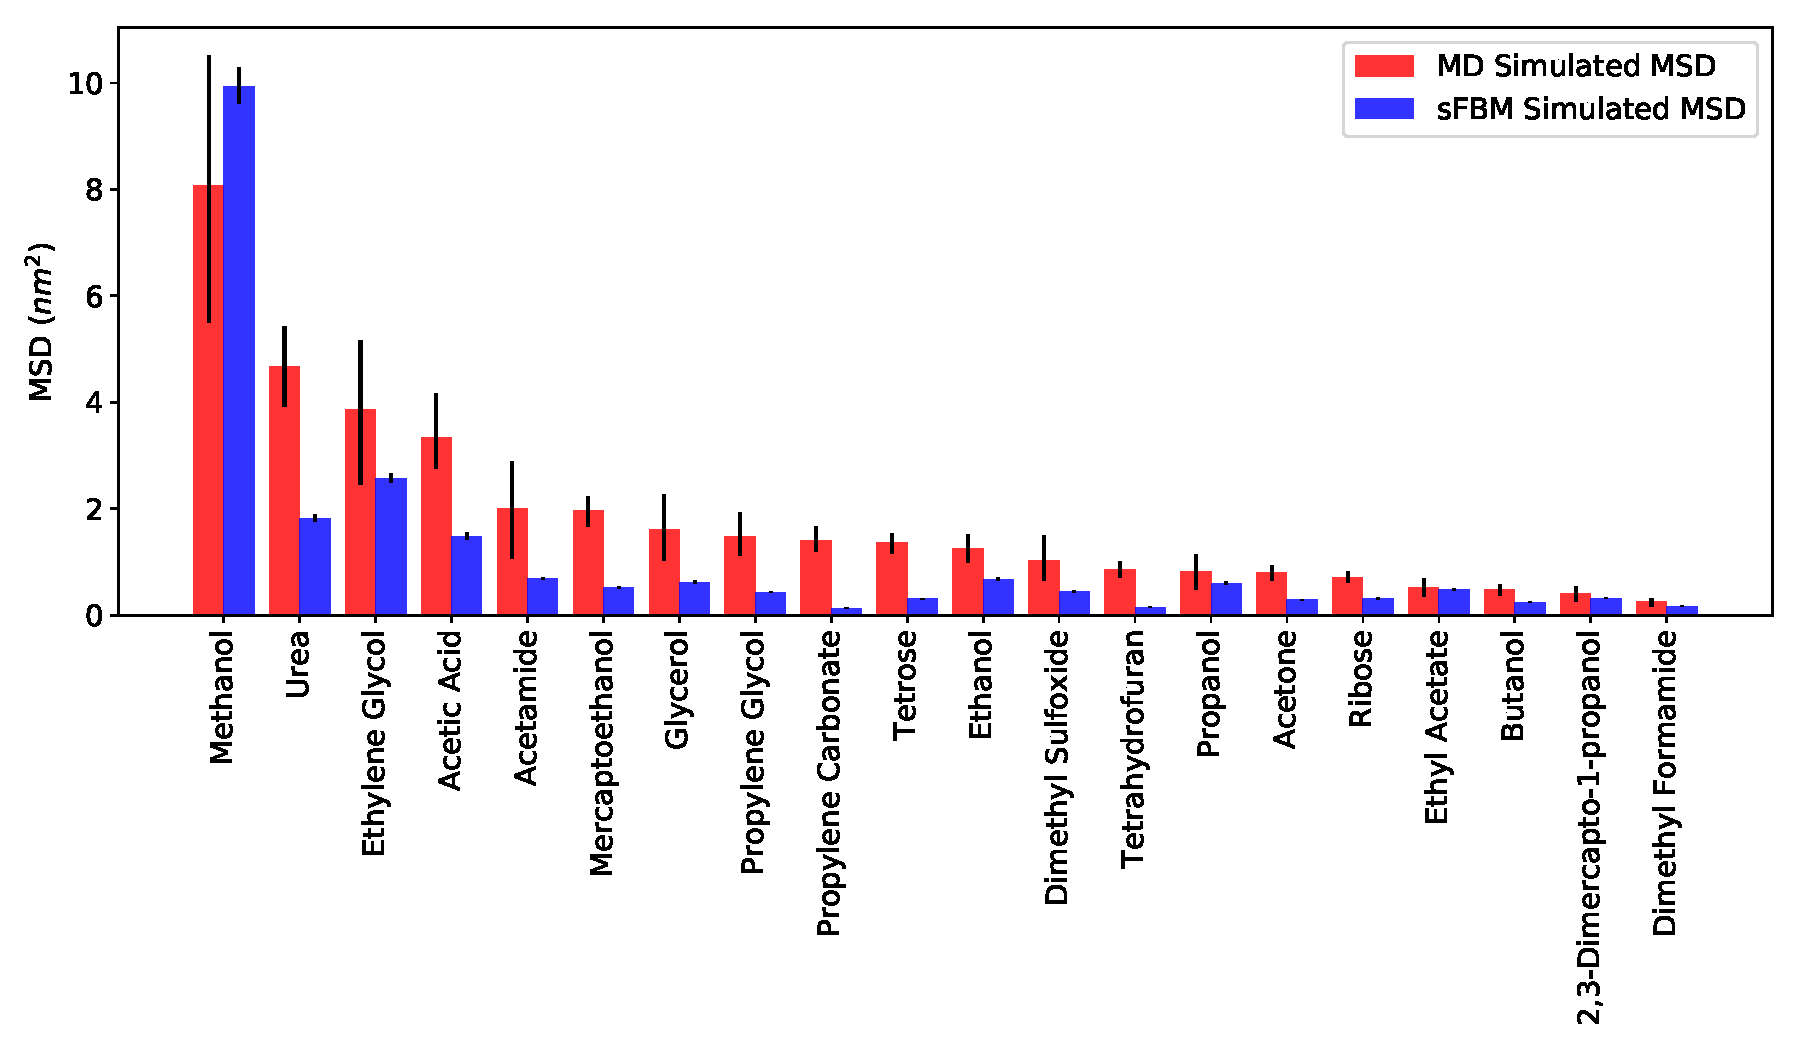
\includegraphics[width=\textwidth]{all_emsds.pdf}
  \caption{}\label{fig:all_msds}
  \end{figure}

  \subsection{Markov State Model Fits}\label{section:msm_results}
  
  The emission distributions are non-Gaussian and heavy-tailed (see Figure~\ref{fig:emissions_MET}).
  \begin{itemize}
    \item The heavy tails of the distribution are a consequence of hopping.
    \item Heavily sampled states fit well to L\'evy stable distributions.
    \item The rarer states have less data, but we still assume L\'evy stable distributions.
  \end{itemize}
  
  % BJC: worth proving these are non-Gaussian? One might argue that they look Gaussian but they are not at all.
  % MRS: there are some simple statistical tests for Gaussianness you can use.  Also might br good to put the 
  % parameters with the plots, as it's hard to tell how different they may or may not be.
  \begin{figure}[!h]
  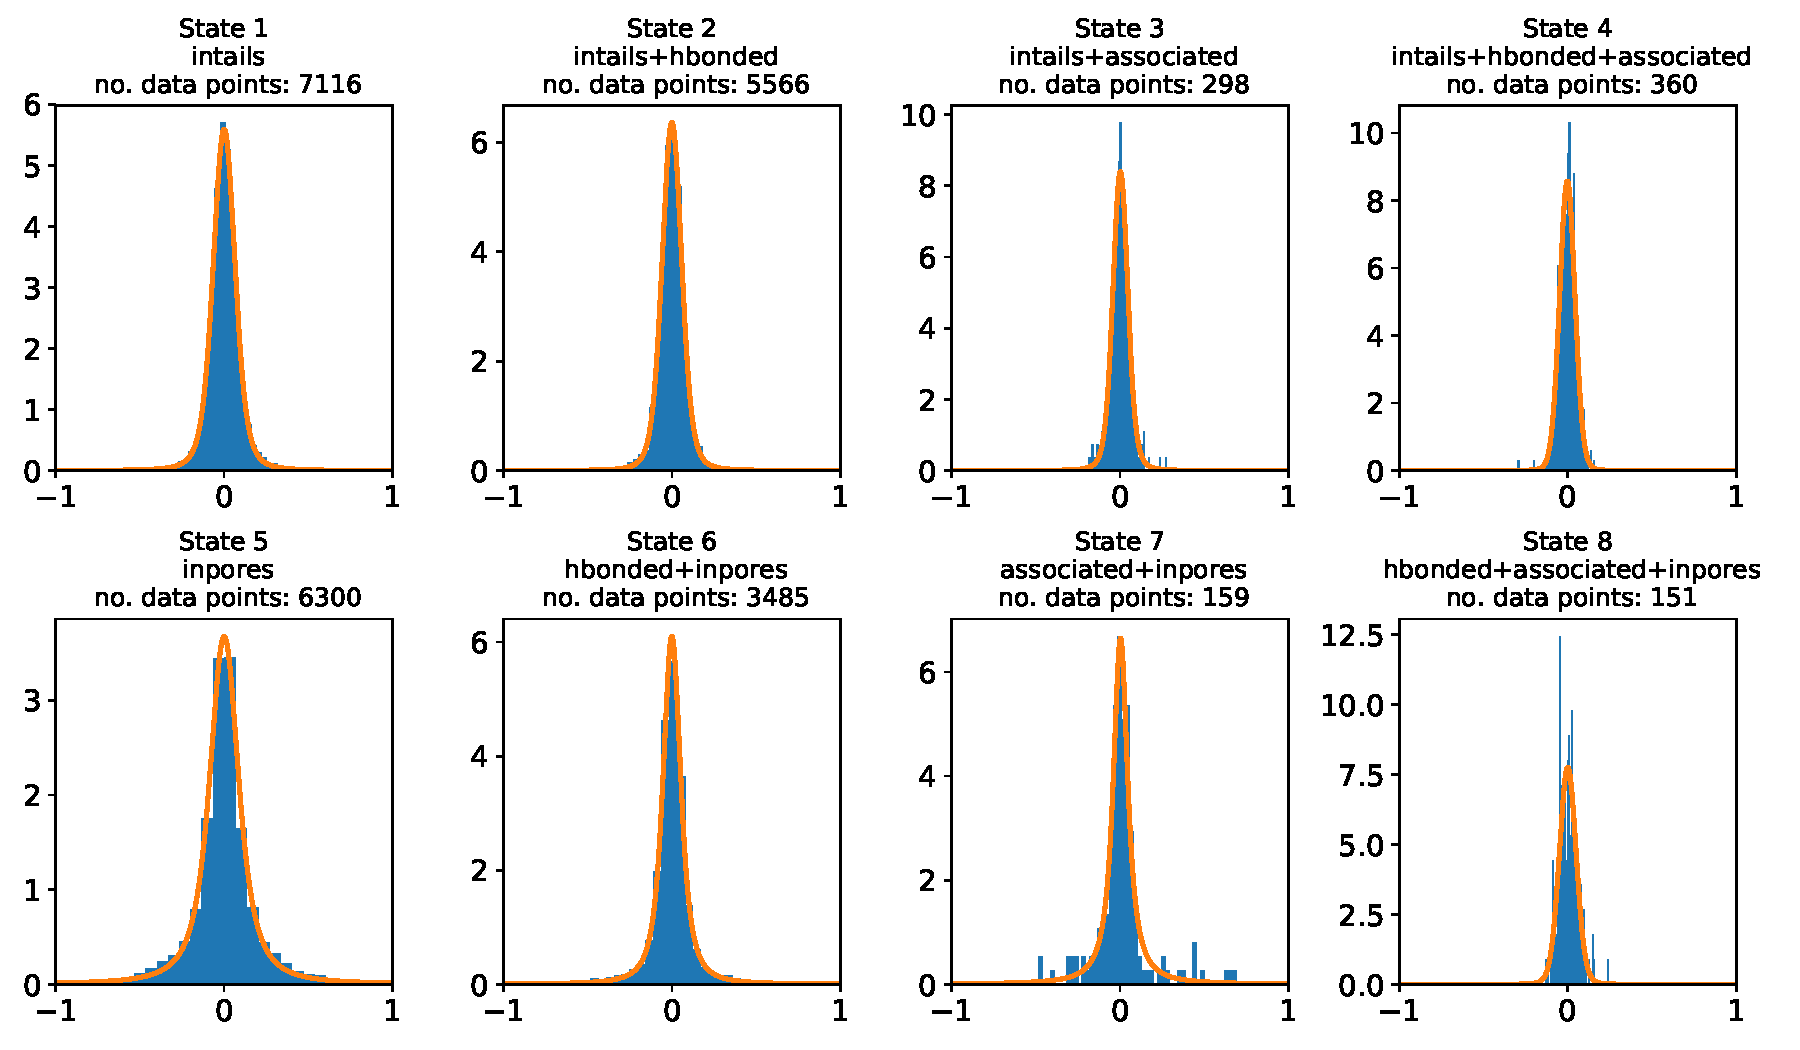
\includegraphics[width=\textwidth]{emissions_MET.pdf}
  \caption{}\label{fig:emissions_MET}
  \end{figure}

  % BJC: need better or more descriptive way of describing stochastic simulations
  % BJC: or could say that whenever we say simulations, we mean stochastic simulations unless it is specified as a molecular dynamics simulation.
  % MRS: could say timeseries simulation?  MD is stochastic as well.
  Simulating solute trajectories (see Section~\ref{method:MSMs}) by drawing independent  
  observations from the emission distributions yields near linear MSD curves
  with final values that are far higher than those observed in our molecular simulations.
  \begin{itemize}
	% BJC: right number of solute trajectories to simulate for comparison? More tightens the error bars
    \item In the case of methanol, the final MSD value is about 25x higher than that observed in our
    previous transport study (see Figure~\ref{fig:msd_MET}).
    \item The linear behavior of the MSD curve is not consistent with subdiffusion.
  \end{itemize}
  %MRS: so, is there a way we should have been able to tell beforrehand that this approach didn't work that we an explain?
  %or can we show we needed to do this to get the results?
  %BJC1: could just show autocorrelation function of all increments, which has negative dip at k=1 
  \begin{figure}[!h]
  \centering
  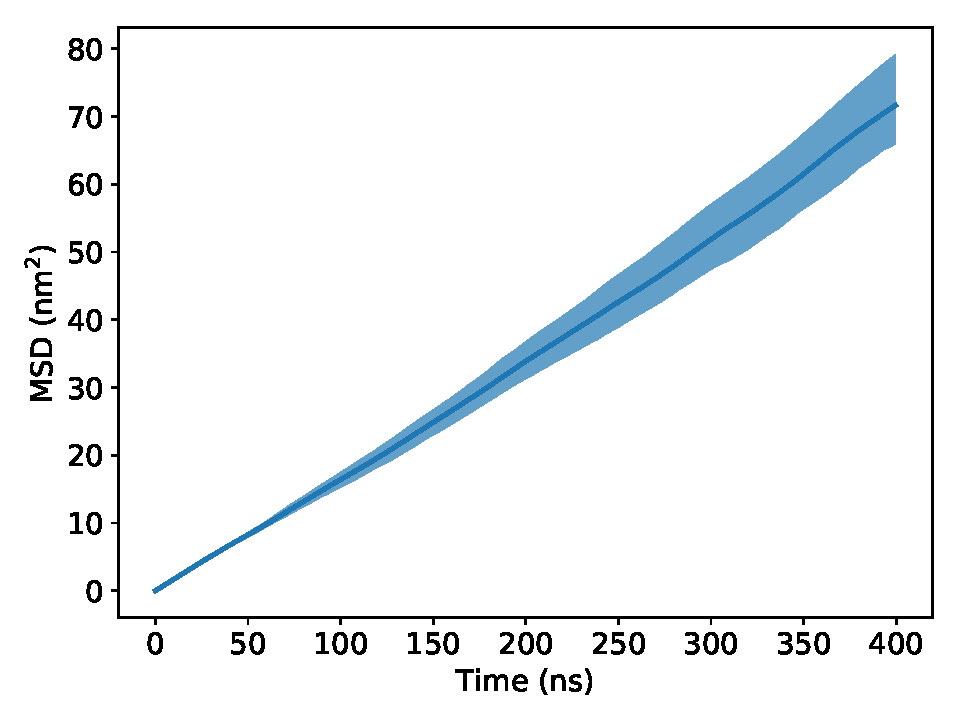
\includegraphics[width=0.5\textwidth]{MET_msd.pdf}
  \caption{}\label{fig:msd_MET}
  \end{figure}
  
  \noindent Anti-correlation between hops may be responsible for subdiffusive behavior.
  \begin{itemize}
    \item In general, we observe negative correlation between hops.
    \item A L\'evy driven OU process may be a more appropriate way to model
    the stochastic dynamics of this system since you can incorporate autocorrelation.
    \item Extracting reliable correlation functions is difficult with our data
    due to relatively frequent switching resulting in sets of short disjoint time 
    series describing each state.
    % \item Therefore we did not do this and attempted to fit a different model. 
    %BJC: we could add some artificial correlation to prove the anti-correlation hypothesis
  \end{itemize}

  \section{Conclusion}
  
  We have tested two different mathematical frameworks for describing solute
  motion in an H\textsubscript{II} phase LLC membrane.
  \begin{itemize}
    \item Markov state modeling with predefined states gives a nice description
    of transitions between observed states as well as the type of stochastic 
    behavior shown in each state. However, it doesn't accurately portray correlated
    time series behavior leading to overpredicted MSDs.
    \item Subordinated fractional Brownian motion has a nice theoretical foundation
    in the anomalous diffusion literature. A two mode model that describes dynamics
    based on whether a solute is in or out of the pore region leads to MSDs fairly
    consistent with MD simulated trajectories.
  \end{itemize}
 
  \section*{Supporting Information}

  Detailed explanations and expansions upon the results and procedures mentioned in
  the main text are described in the Supporting Information. This information is
  available free of charge via the Internet at http://pubs.acs.org.

  \section*{Acknowledgements}

  Molecular simulations were performed using the Extreme Science and
  Engineering Discovery Environment (XSEDE), which is supported by National
  Science Foundation grant number ACI-1548562. Specifically, it used the Bridges
  system, which is supported by NSF award number ACI-1445606, at the Pittsburgh
  Supercomputing Center (PSC). This work also utilized the RMACC Summit supercomputer,
  which is supported by the National Science Foundation (awards ACI-1532235 and
  ACI-1532236), the University of Colorado Boulder, and Colorado State
  University. The Summit supercomputer is a joint effort of the University of
  Colorado Boulder and Colorado State University.

  \clearpage

  \bibliographystyle{ieeetr}
  \bibliography{stochastic_transport}

  \newpage

  \section*{TOC Graphic}

\end{document}
